%------------------------------------------------------------------------------
% Author(s):
% Varaun Ramgoolie
%
% Copyright:
%  Copyright (C) 2020 Brad Bachu, Arjun Mohammed, Varaun Ramgoolie, Nicholas Sammy
%
%  This file is part of Applied-Mathematics-Unit2 and is distributed under the
%  terms of the MIT License. See the LICENSE file for details.
%
%  Description:
%     Year: 2009 
%     Module: 3
%     Question: 5
%------------------------------------------------------------------------------

%------------------------------------------------------------------------------
% 5 a
%------------------------------------------------------------------------------

\begin{subquestions}
	
\subquestion

\textbf{\textit{Sketch and Translate:}} \\ \\
\begin{figure}[H]
	\begin{center}
		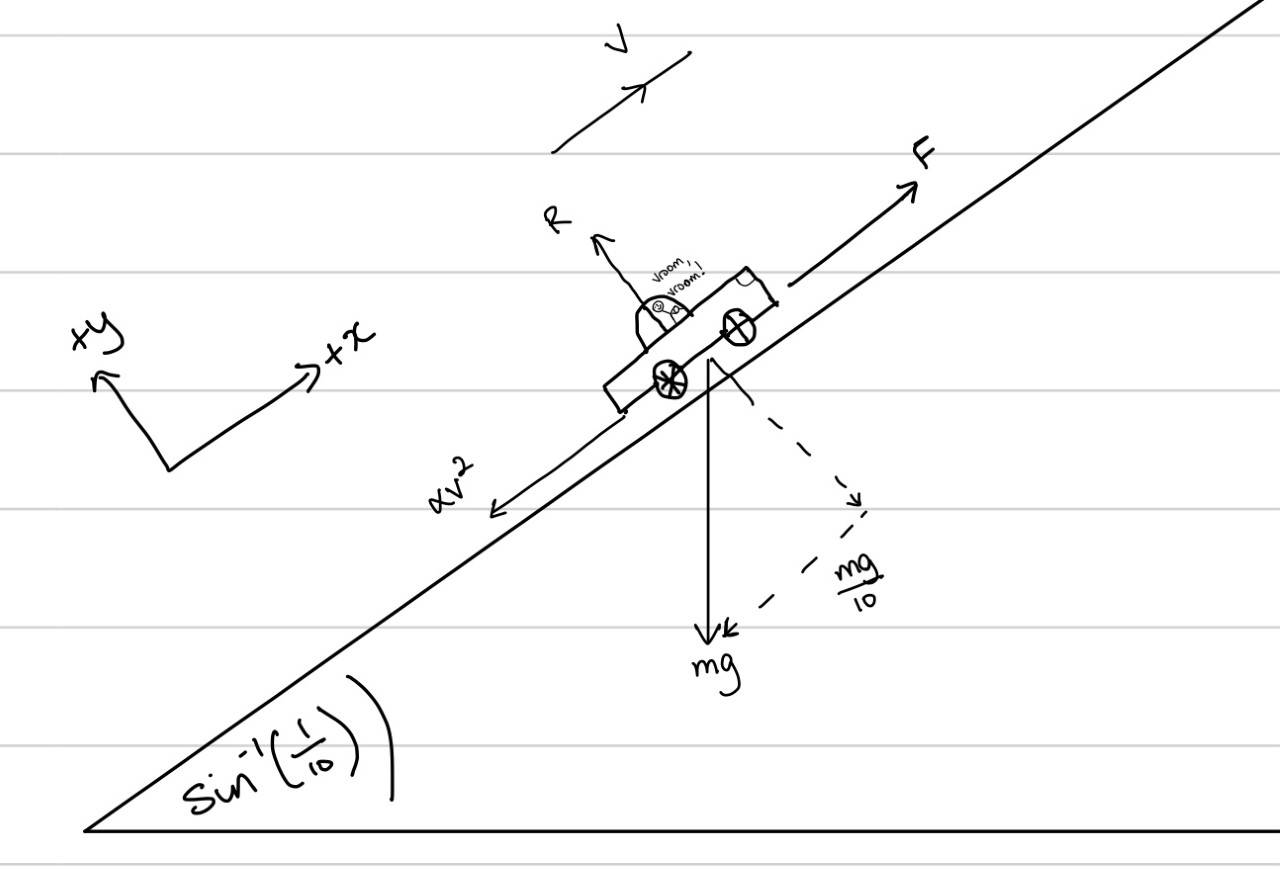
\includegraphics[scale=0.25]{../2009/figures/2009q5-1}
		\caption{\label{2009:q5:Sketch1} Car moving uphill.}
	\end{center}
\end{figure}
We are given the motion of a vehicle moving up a inclined plane, against a resistive force. As the car is given to be moving at a steady speed, the acceleration is 0. Since the frictional resistance, $\vec{F_f}$, is proportional to the square of the speed, we can express this as $|\vec{F_f}| = kv^2$.
	

	
	
\textbf{\textit{Simplify and Diagram:}} \\ \\	
\begin{figure}[H]
	\begin{center}
		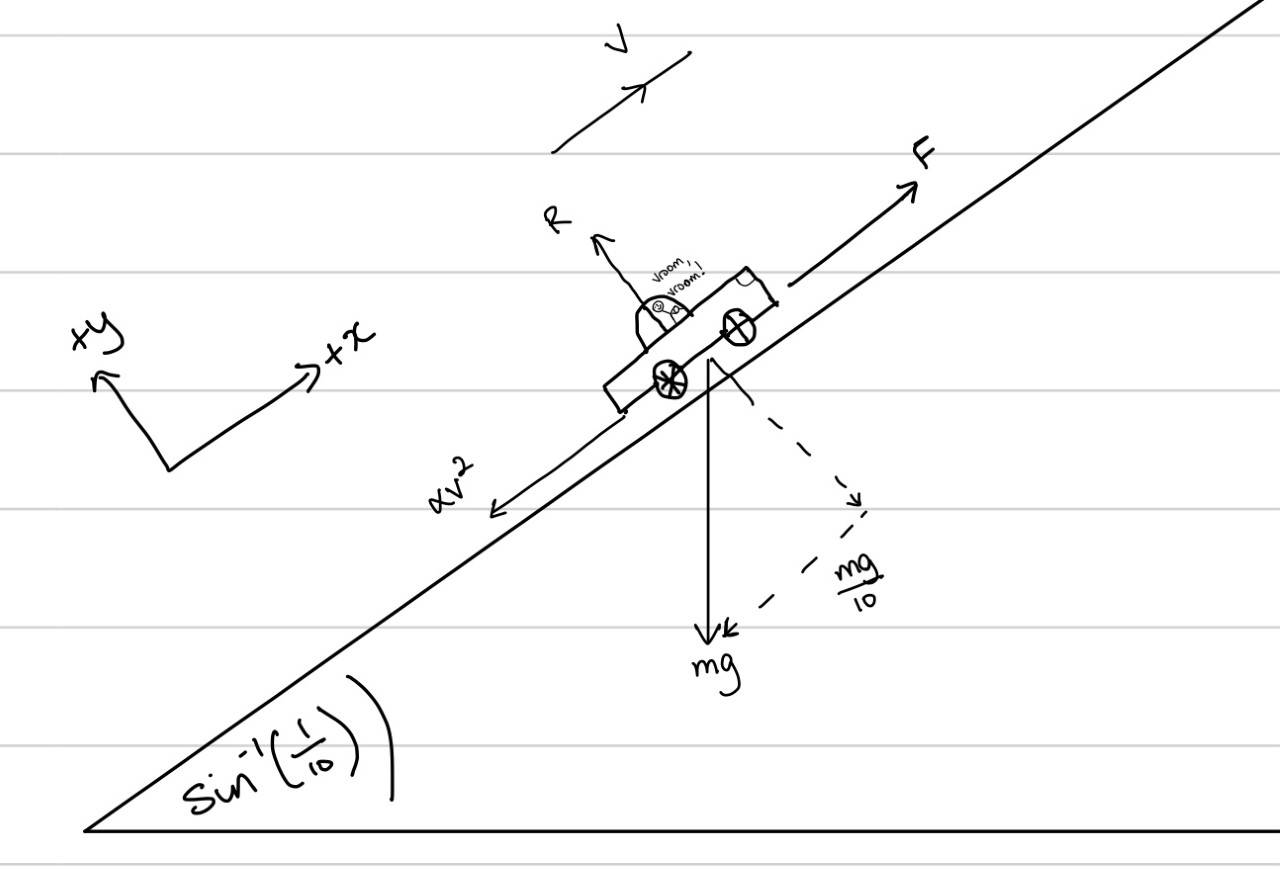
\includegraphics[scale=0.25]{../2009/figures/2009q5-1}
		\caption{\label{2009:q5:Diagram1} Car moving uphill.}
	\end{center}
\end{figure}

As the acceleration of the vehicle is 0, we know that (from Newton's Second Law) there is no resultant force on the vehicle. Therefore, we can resolve our forces and use our knowledge of tractive force to find the power exerted by the vehicle. We will define the following forces as:
\begin{itemize}
	\item $\vec{F_T}$ which is the tractive force,
	\item $\vec{W}$ which is the weight of the car,
	\item $\vec{F_f}$ which is the frictional force,
	\item $\vec{R}$ which is the normal reaction force.
\end{itemize}
The subscripts $x$ and $y$ indicate whether the value that it is attached to is a component in the horizontal or vertical direction.


\textbf{\textit{Represent Mathematically:}} \\ \\
Firstly, we will resolve our forces as, \TODO{magW isntead of mg and vec(a)=vec0}
\begin{align}
	\vec{F_T} & = |\vec{F_T}|\xhat \\
	\vec{W} & = -|\vec{W}|\sin\left(\arcsin\left(\frac{1}{10}\right)\right)\xhat -|\vec{W}|\cos\left(\arcsin\left(\frac{1}{10}\right)\right)\yhat \nn \\
	        & = -\frac{mg}{10}\xhat - mg\cos\left(\arcsin\left(\frac{1}{10}\right)\right)\yhat \\
	\vec{F_f} & = -|\vec{F_f}|\xhat \\
	\vec{R} & = |\vec{R}|\yhat \,.
\end{align}

From Newton's Second Law, we get that,
\begin{align}
	\sum \vec{F} & = \vec{0} \nn \\
	\sum \left(F_x \hat{x} + F_y \hat{y}\right) &= 0 \hat{x} + 0 \hat{y} 
\end{align}
Hence,
\begin{align}
	\sum F_x & = 0 \label{2009:q5:FxEqn1} \\
	\text{and} & \nn \\
	\sum F_y & = 0 \,.
\end{align}
where $F_x$ and $F_y$ are the components of the forces in the $x$ and $y$ directions respectively.

Finally, we will use,
\begin{equation}
	\text{Power, }P = |\vec{F_T}|\times v \label{2009:q5:PEqn1} \,.
\end{equation}




\textbf{\textit{Solve and Evaluate:}} \\ \\
Firstly, as we are given that the frictional force is proportional to the square of the speed of the car and it is equal to 650N when the speed is 25ms$^{-1}$, we get that,
\begin{align}
	|\vec{F_f}| & \propto v^2 \nn \\
	\implies |\vec{F_f}| & = kv^2, \nn \\
	650 & = 25^2k \nn \\
	\implies k & = \frac{26}{25} \,.
\end{align}

From \req{2009:q5:FxEqn1}, we get that,
\begin{align}
	\sum F_x = |\vec{F_T}|-\frac{mg}{10}-|\vec{F_f}| & = 0 \nn \\
	|\vec{F_T}| & = \frac{mg}{10}+|\vec{F_f}| \nn \\
	            & = \frac{750\times10}{10} +650 \nn \\
	            & = 1400N \,. \label{2009:q5:TracEqn1}
\end{align} 

Finally, substituting our values into \req{2009:q5:PEqn1}, we get that,
\begin{align}
	P & = 1400 \times 25 \nn \\
	  & = 35000W \,.
\end{align}

%------------------------------------------------------------------------------
% 5 b
%------------------------------------------------------------------------------

\subquestion
	
\begin{subsubquestions}
	
\subsubquestion

\textbf{\textit{Sketch and Translate:}} \\ \\
\begin{figure}[H]
	\begin{center}
		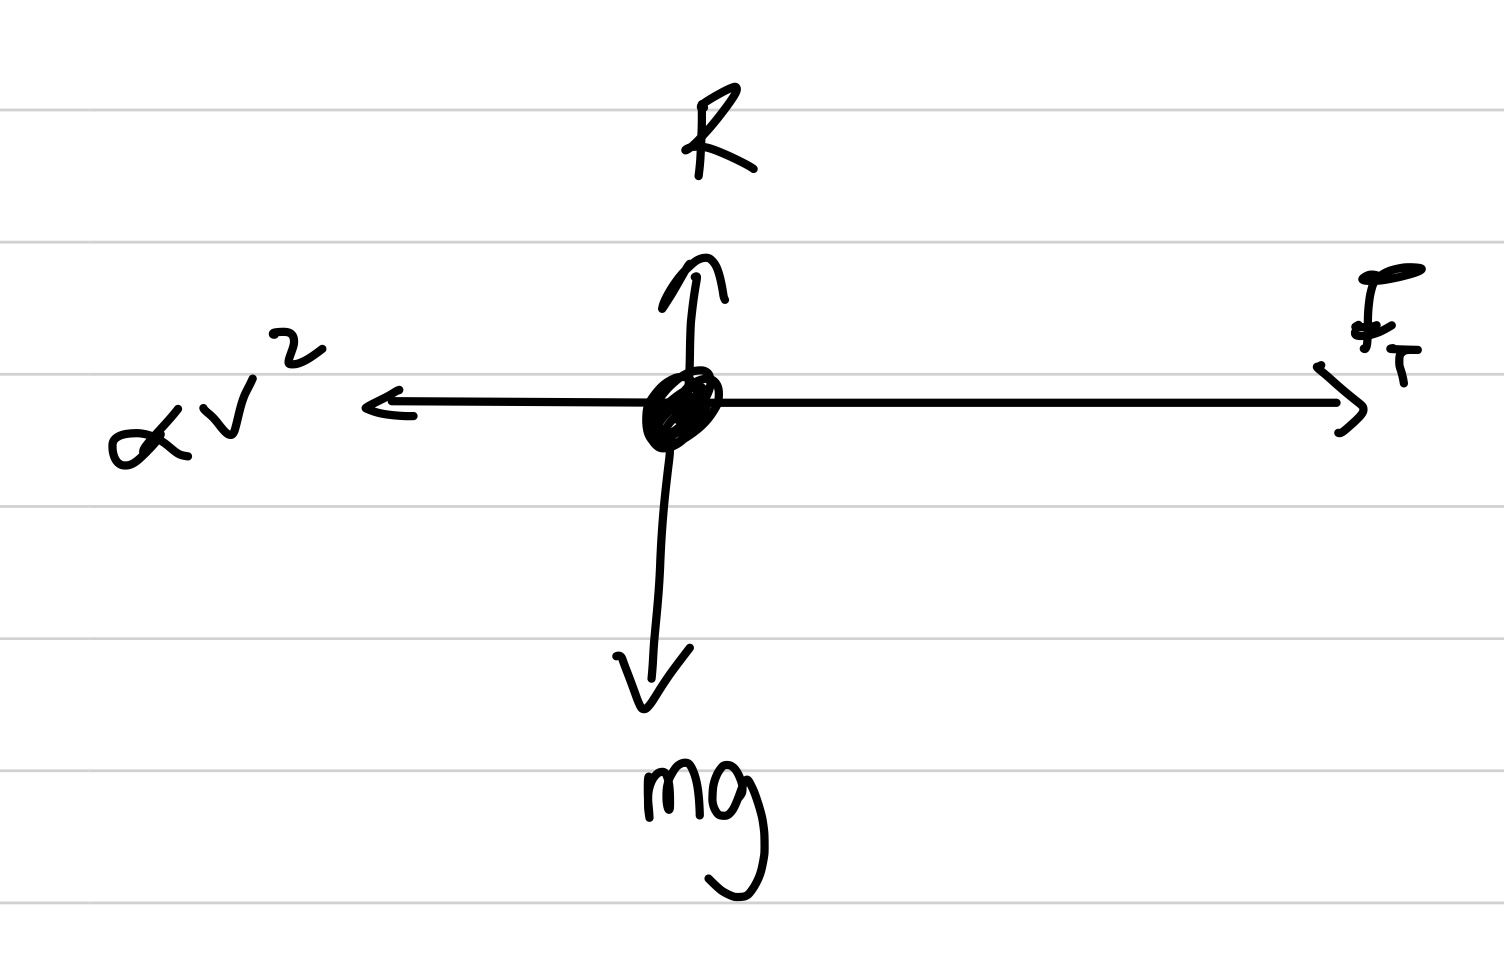
\includegraphics[scale=0.25]{../2009/figures/2009q5-2}
		\caption{\label{2009:q5:Sketch2} Car on flat ground.}
	\end{center}
\end{figure}	
As the car is now on flat ground, it does not experience any resistance to motion against gravity. 




\textbf{\textit{Simplify and Diagram:}} \\ \\
\begin{figure}[H]
	\begin{center}
		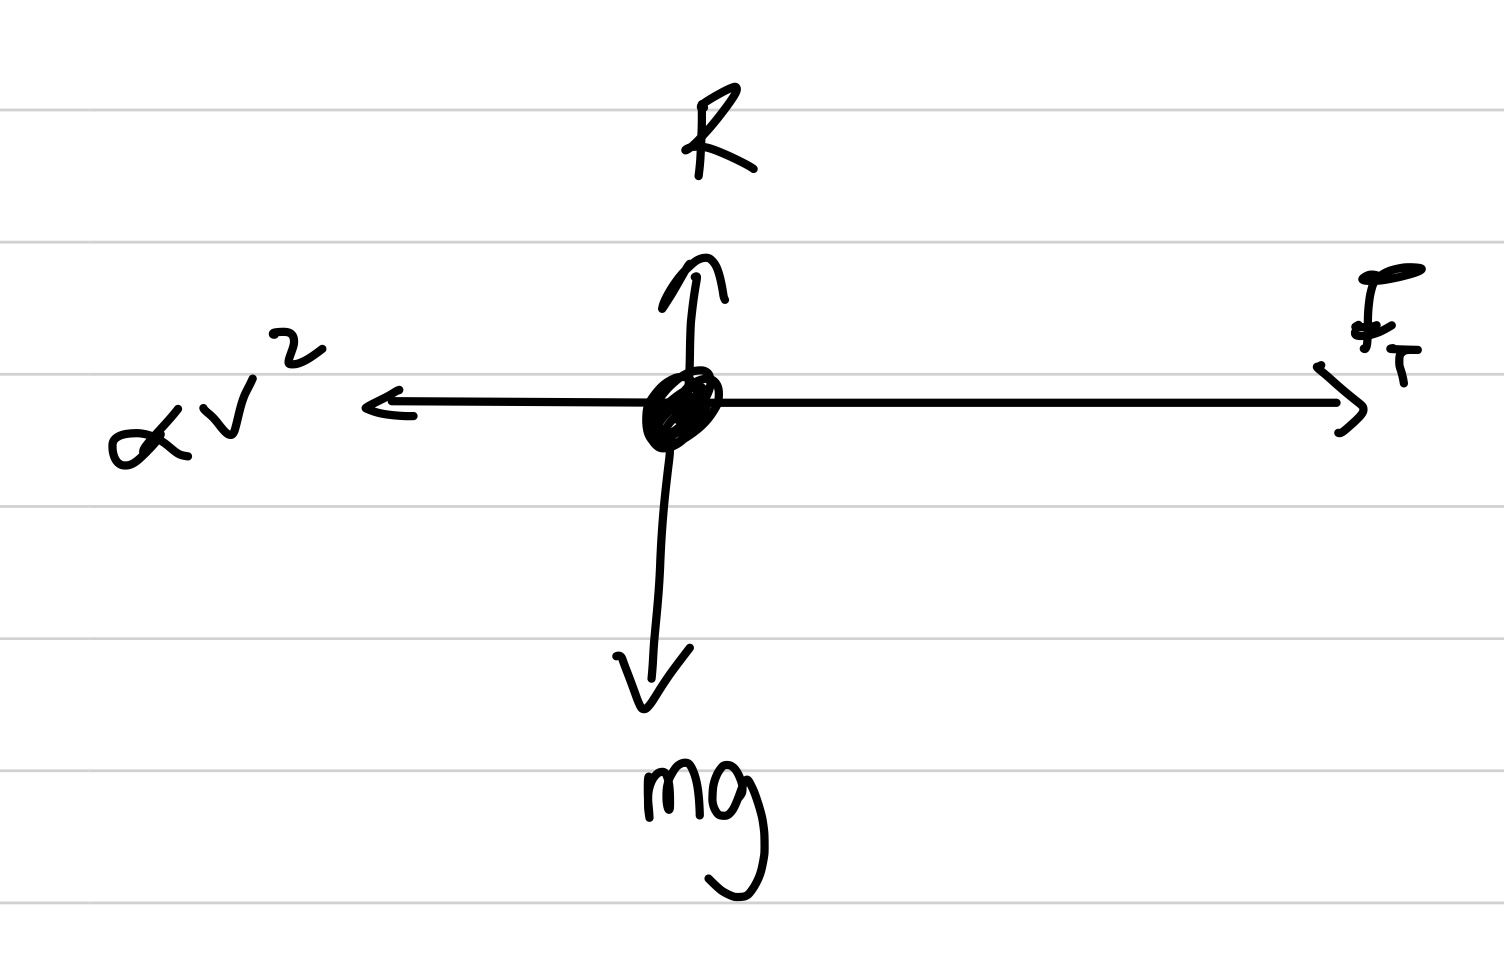
\includegraphics[scale=0.25]{../2009/figures/2009q5-2}
		\caption{\label{2009:q5:Diagram2} Car on flat ground.}
	\end{center}
\end{figure}	
As we are given that the power exerted by the engine is the same, we can find the resultant force on the body (by Newton's Second Law) and find its initial acceleration. We will use the same forces defined in (a). We will take the immediate velocity of the vehicle at the level road as 25ms$^{-1}$.
We will again define:
\begin{itemize}
	\item $a_x$ to be the acceleration of the car in the $x$-direction.
\end{itemize}



\textbf{\textit{Represent Mathematically:}} \\ \\
Firstly, we will resolve our forces as,
\begin{align}
	\vec{F_T} & = |\vec{F_T}|\xhat \\
	\vec{W} & = -|W|\yhat \\
	\vec{F_f} & = -|\vec{F_f}|\xhat \\
	\vec{R} & = |\vec{R}|\yhat \,.
\end{align}

From Newton's Second Law, we know that,
\begin{equation}
	\sum F_x = ma_x \label{2009:q5:FxEqn2} \,.
\end{equation}
where $F_x$ is the component of the forces in the $x$ direction.




\textbf{\textit{Solve and Evaluate:}} \\ \\
Substituting our values into \req{2009:q5:FxEqn2}, we get that,
\begin{align}
	\sum F_x = |\vec{F_T}|-|\vec{F_f}| & = ma_x \nn \\
	           1400 - 650 & = 750a_x \nn \\
	           \implies a_x & = 1 ms^{-2} \,.
\end{align}

%------------------------------------------------------------------------------

\subsubquestion
\textbf{\textit{Sketch and Translate:}} \\ \\
\begin{figure}[H]
	\begin{center}
		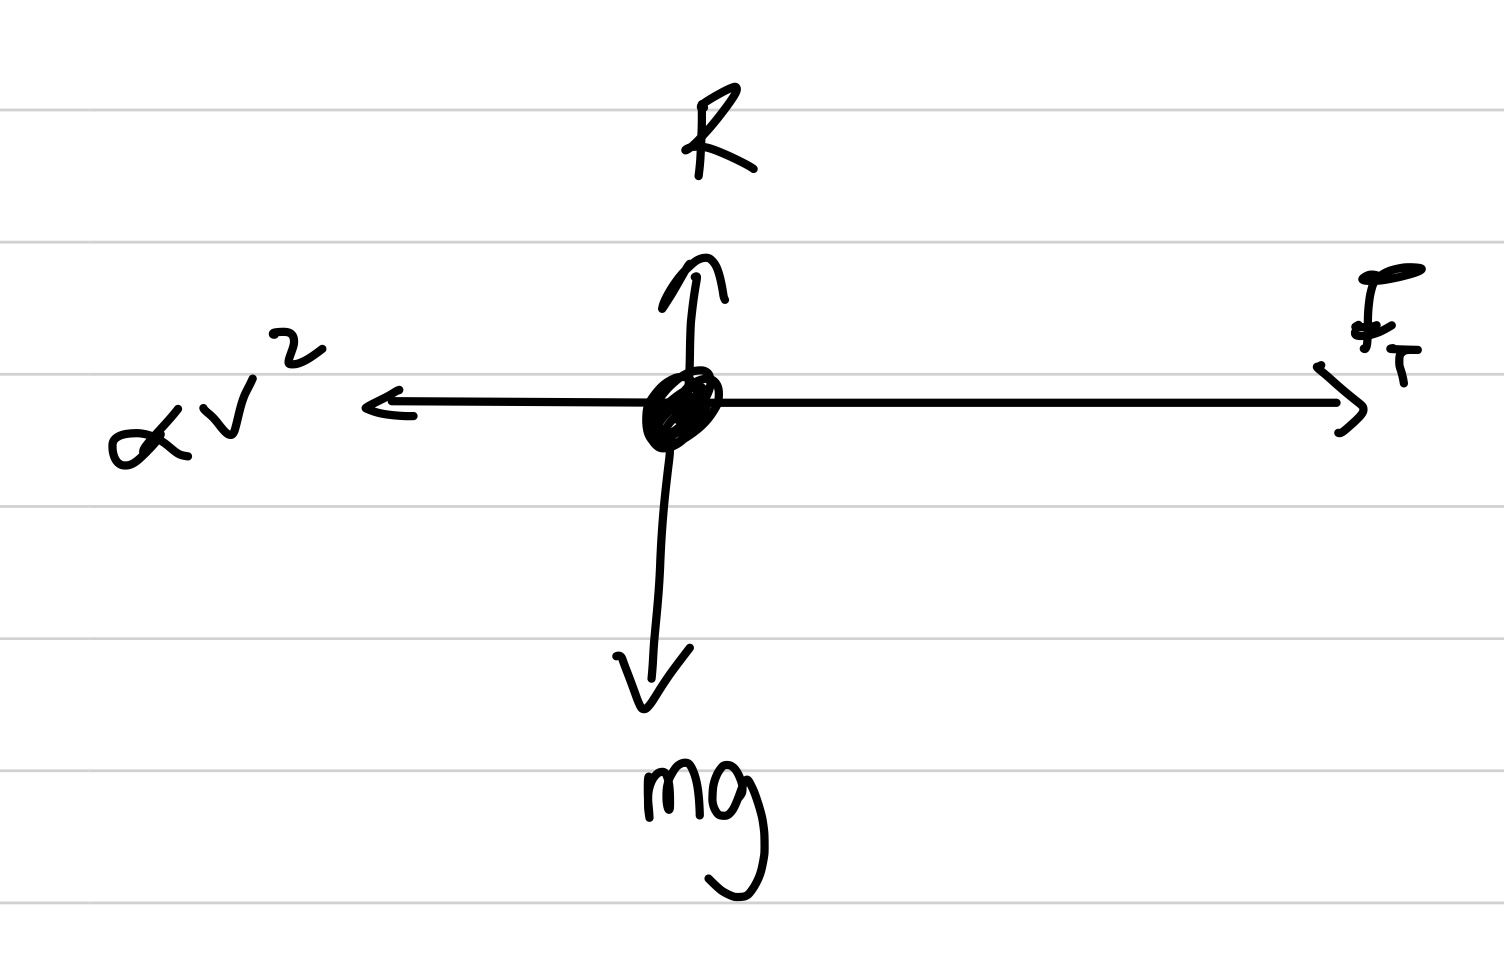
\includegraphics[scale=0.25]{../2009/figures/2009q5-2}
		\caption{\label{2009:q5:Sketch3} Car on flat ground.}
	\end{center}
\end{figure}	
We should notice that the maximum speed will occur when the acceleration of the car is 0.




\textbf{\textit{Simplify and Diagram:}} \\ \\
\begin{figure}[H]
	\begin{center}
		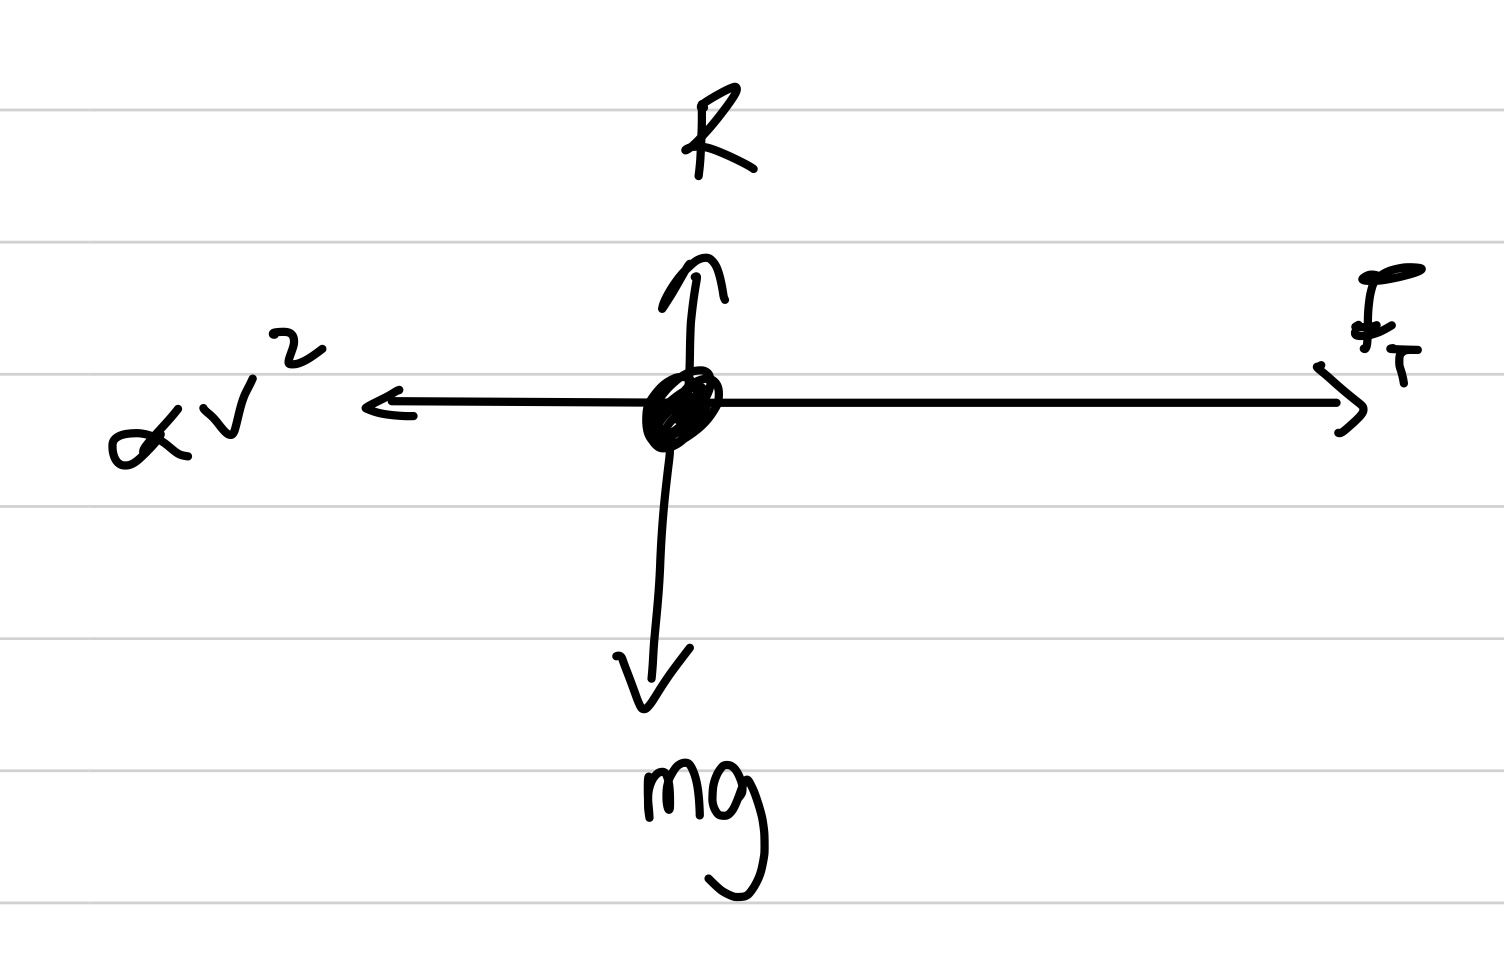
\includegraphics[scale=0.25]{../2009/figures/2009q5-2}
		\caption{\label{2009:q5:Diagram3} Car on flat ground.}
	\end{center}
\end{figure}	
As we have found in (b)(i) that the initial acceleration of the car is positive, the frictional resistance of the car will increase as the velocity will increase. Thus, in order to find the maximum velocity, we need to find the point where the frictional resistance is equal to the tractive force.\footnote{This is from \req{2009:q5:FxEqn2}. When both are equal, $a_x$ must be 0.} It is also worth noting that the power exerted by the engine is constant (35000W).




\textbf{\textit{Represent Mathematically:}} \\ \\
We know that the frictional force is expressed as,
\begin{equation}
	|\vec{F_f}| = \frac{26}{25}v^2 \,.
\end{equation}

Again, from Newton's Second Law, we know that,
\begin{equation}
	\sum F_x = ma_x \label{2009:q5:FxEqn3} \,.
\end{equation}
where $F_x$ is the component of the forces in the $x$ direction and $a_x$ the acceleration in the $x$ direction.

Finally, we also know that, \TODO{dont make subject too early}
\begin{align}
	P & = |\vec{F_T}|\times v \label{2009:q5:PEqn2} \nn \\
	\implies |\vec{F_T}| & = \frac{P}{v} \,. 
\end{align}
	



\textbf{\textit{Solve and Evaluate:}} \\ \\
Substituting our values into \req{2009:q5:FxEqn3}, we get,
\begin{align}
	\sum F_x & = ma_x \nn \\
	|\vec{F_T}|-|\vec{F_f}| & = m(0) \nn \\
	\frac{35000}{v} - \frac{26}{25}v^2 & = 0 \nn \\
	\implies v & = \sqrt[3]{\frac{35000}{\frac{26}{25}}} \nn \\
	           & = 32.3 ms^{-1} \,.
\end{align}

\end{subsubquestions}
	
\end{subquestions}










